\graphicspath{{img/results}{img/results/out}}

\chapter{Results}
\label{ch:results}
This chapter will present the results of the smarticle experiments in the TASEP. We will start by setting a baseline with the classical TASEP and analyze how different speed distributions affect this purely stochastic system. Next, we will compare the results with a simple hard-coded policy, before moving on to the smarticle training. We will analyze the results of the smarticle training for different reward structures and compare them to the baseline. 


\section{Setting a Baseline: Classical TASEP}
\label{sec:baseline}
\begin{wrapfigure}{R}{0.45\textwidth}
    \raisebox{0pt}[\dimexpr\height-0.6\baselineskip\relax]{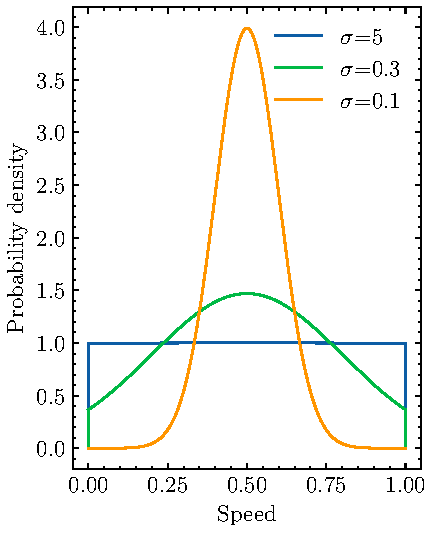
\includegraphics{truncated_normal_small.pdf}}
    \caption{Normalized truncated normal distributions with mean $\mu=0.5$ and different standard deviations $\sigma$.}
    \label{fig:speed_dists}
\end{wrapfigure}
This section will use the classical 2D (T)ASEP as introduced in section \ref{sec:2d-tasep}. We will make it totally asymmetric in the horizontal direction (the \textit{forward} direction) by setting the probability $p$ to jump forward to $1/2$ and the probability $q$ to jump backward to $0$. The vertical direction (the \textit{up/down} direction) will be symmetric with probabilities $a=b=1/4$. The system has periodic boundary conditions in both directions. We will analyze a $128 \times 32$ system and a narrower $128 \times 6$ system. Both systems will be initialized with a checkerboard pattern of particles and holes, yielding a density of $\rho = 1/2$. This density will be chosen for most experiments, as it is dense enough for the different policies and speed distributions to have a significant effect on the system, but not so dense that the system is always jammed. Speeds will be drawn from a truncated normal distribution with mean $0.5$ and different standard deviations $\sigma$. The distribution is truncated at $0$ and $1$, so that speeds are always in that range. Two example speed distributions are shown in figure \ref{fig:speed_dists}. 

\subsection{Finding the Steady State}
\begin{figure}[h]
    \centering
    \begin{subfigure}{\textwidth}
        \centering
        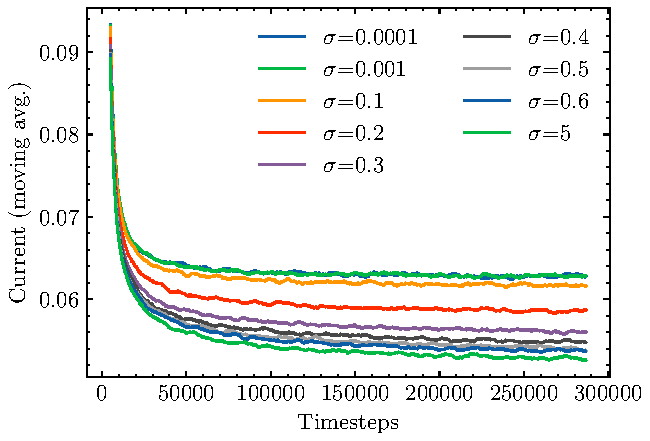
\includegraphics{currents_fixed_sigma_128x32}
        \caption{System size: 128x32}
        \label{fig:currents_fixed_sigma_128x32}
    \end{subfigure}
    \par\vspace{1cm}
    \begin{subfigure}{\textwidth}
        \centering
        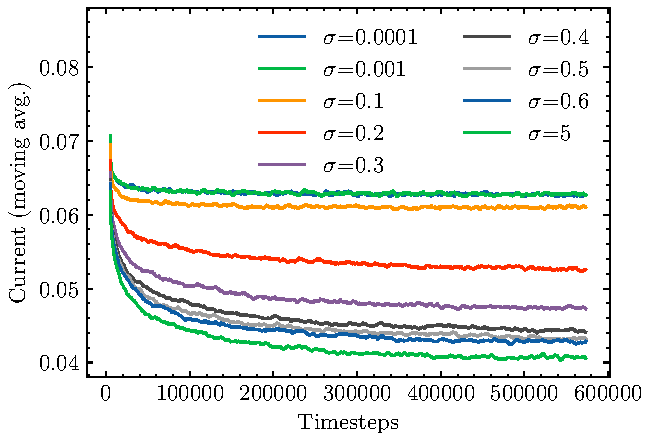
\includegraphics{currents_fixed_sigma_128x3}
        \caption{System size: 128x3}
        \label{fig:currents_fixed_sigma_128x3}
    \end{subfigure}
    \caption{Current as a function of time steps since initialization of the system to the checkerboard pattern for different speed distribution standard deviations $\sigma$ and two different system sizes. The data is averaged over 800 independent runs and plotted with a moving average over 5000 time steps.}
\end{figure}
When we want to compare the average current of different ASEP configurations, we have to make sure that the system has reached a steady state. The steady state has been reached when the current fluctuates around a constant mean value without an overall upwards or downwards trend. The time it takes to reach the steady state depends on the system size, the density and the initial conditions. When using a checkerboard setup for example, it's intuitive that the current will be very high in the beginning of the simulation, as every particle has an empty site in front of it and can move forward. As time passes, the probability of being able to move forward decreases (for different reasons that we will examine in the next paragraphs), and the mean current drops. 
\\
\\
Figures \ref{fig:currents_fixed_sigma_128x32} and \ref{fig:currents_fixed_sigma_128x3} show the current as a function of time steps since initialization of the system to the checkerboard pattern for different speed distribution standard deviations $\sigma$. We can see that for small $\sigma$, when all particles have similar speeds, the current converges quickly and reaches a steady state after about 100,000-150,000 time steps. For larger $\sigma$, particles have different speeds and the equilibration phase takes longer, as jams form and dissolve and slow particles move very rarely. For $\sigma = 5$, especially in the narrow system (Fig. \ref{fig:currents_fixed_sigma_128x3}), we see that the steady state is still not quite reached after 300,000 time steps. 
\\
For the following experiments, the steady state current will be calculated by running the simulation for 600,000 time steps and averaging the current over the last 150,000 time steps. This ensures that the system has reached a steady state even for the configurations that take longer to equilibrate.

\begin{figure}
    \centering
    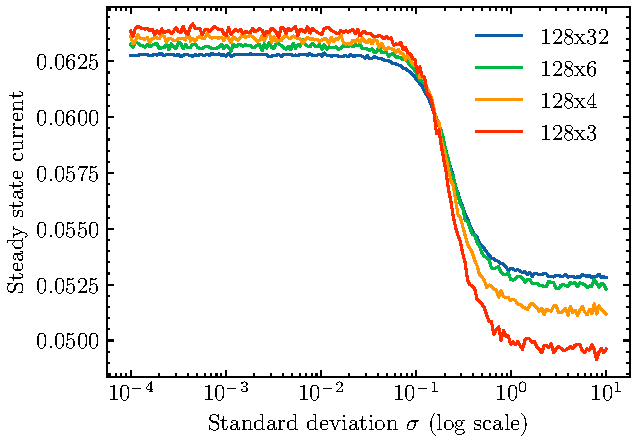
\includegraphics{steady_state_current_sizes_log.pdf}
    \caption{Steady state current as a function of the speed distribution's standard deviation $\sigma$ for different system sizes. Steady state current is calculated as the average current over all remaining time steps after the steady state has been reached (the current has stopped dropping). The data is averaged over 800 independent runs.}
    \label{fig:steady_state_current_sizes_log}
\end{figure}

\begin{figure}
    \centering
    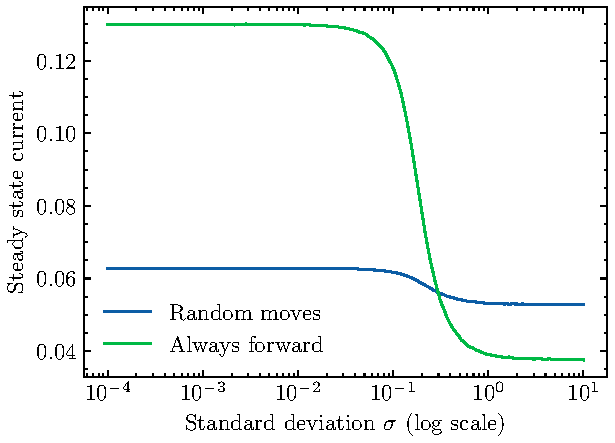
\includegraphics{steady_state_current_both_log.pdf}
    \caption{Steady state current as a function of the speed distribution's standard deviation $\sigma$ for two different ASEP configurations. \enquote{Random moves} has a probability of $p=1/2$ to move forward probabilities $a=b=1/4$ to move up/down. \enquote{Always forward} has $p=1$ and $a=b=0$. A system of size 128x32 was used. The data is averaged over 800 independent runs.}
    \label{fig:steady_state_current_always_forward}
\end{figure}
